\documentclass[10pt]{article}
\usepackage[english]{babel}
\usepackage{../../../meta-inf/lib/naproche}
\usepackage{amssymb}
\usepackage{mathtools} % for \coloneq

\usepackage{stex-highlighting}
\providebool{emph} % "\newbool{emph}" does not work...
\setbool{emph}{false}
\colorlet{emphcolor}{violet}
\let\oldemph\emph
\renewcommand\emph[1]{\setbool{emph}{true}\ifbool{forthel}{\textcolor{emphcolor}{\itshape#1}}{\oldemph{#1}}\setbool{emph}{false}}
\renewcommand{\varemph}[1]{\ifbool{emph}{\textcolor{emphcolor}{#1}}{\textcolor{black}{#1}}}

\usepackage[right=6cm,left=3cm,bottom=3cm,marginparwidth=5cm]{geometry}

\usepackage{fancyhdr}
\renewcommand{\sectionmark}[1]{\markboth{#1}{}} 
\def\libarchive{}
\pagestyle{fancy}
\fancyhead[L]{\libarchive}
\fancyhead[C]{\nouppercase\leftmark}  % section title
\fancyhead[R]{\thepage}               % page number
\fancyfoot[C]{}                       % No page number in footer

\usepackage[nobottomtitles]{titlesec}
\titlespacing*{\section}{0pt}{30pt}{0pt}
\titlespacing*{\subsection}{0pt}{30pt}{0pt}
\titlespacing*{\subsubsection}{0pt}{30pt}{0pt}

\documentclass[12pt,oneside]{book}

\usepackage[foundations]{../../lib/tex/naproche}
\usepackage{../../lib/tex/libraries}
\usepackage{graphicx}
\usepackage{float}
\usepackage{caption}
\usepackage{footnote}

\makesavenoteenv{tabular} % Make footnotes work in tabular environments


\title{Foundations of Mathematics}
\author{Marcel Schütz}
\date{2022}

\begin{document}
  \maketitle

  \tableofcontents

  \begin{figure}[H]
    \centering
    \fbox{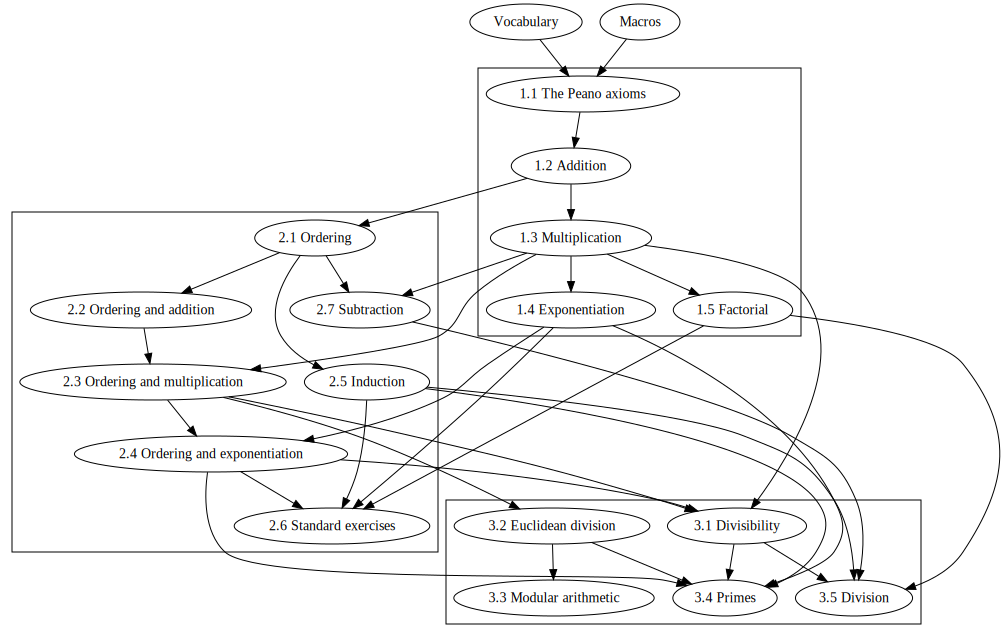
\includegraphics[width=0.9\linewidth]{./dependency-graph/graph.png}}
    \caption*{Interdependencies of the chapters}
  \end{figure}


  \section*{Introduction}

  This is a library providing a foundation of mathematics based on a
  Kelley-Morse like class theory with urelements.
  It introduces common operations on classes like unions or intersections
  (\cref{chapter:classes}) together with detailed proofs of their algebraic
  properties (\cref{chapter:computation-laws-for-classes}), the symmetric
  difference of two classes (\cref{chapter:symmetric-difference}) and the
  notions of ordered pairs and Cartesian products
  (\cref{chapter:pairs-and-products}) as well as proofs of the algebraic
  properties of the latter (\cref{chapter:computation-laws-for-products}).
  Moreover, it provides common operations on maps (\cref{chapter:maps}), various
  properties of images and preimages (\cref{chapter:image-and-preimage}) and the
  notions of injectivity, surjectivity, bijectivity
  (\cref{chapter:injections-surjections-bijections}) and invertibility of maps
  (\cref{chapter:invertible-maps}).
  The library provides an axiom system characterizing sets (\cref{chapter:sets})
  and, furthermore, it covers the notions of binary relations
  (\cref{chapter:binary-relations}), fixed-points of subset preserving maps
  (\cref{chapter:fixed-points}), including and equinumerosity
  (\cref{chapter:equinumerosity}).

  As two famous results it includes the Knaster-Tarski fixed point theorem
  (\cref{FOUNDATIONS_12_8420450166112256}) and the Cantor-Schröder-Bernstein
  theorem (\cref{FOUNDATIONS_13_1913663275401216}).

  \paragraph*{Usage.}
  At the very beginning of each chapter you can find the name of its source
  file, e.g. \path{foundations/sections/01_classes.ftl.tex} for
  \cref{chapter:classes}. This filename can be used to import the chapter via
  \Naproche's \texttt{readtex} instruction to another ForTheL text, e.g.:
  \begin{center}
    \verb`[readtex \path{foundations/sections/01_classes.ftl.tex}]`
  \end{center}

  \paragraph*{Checking times.}
  The checking times for each of the chapters may vary from computer to
  computer, but on mid-range hardware they are likely to be similar to those
  given in table below:

  \begin{center}
    \begin{tabular}{c|c|c}

      & \multicolumn{2}{c}{\textbf{Checking time}}
      \\
      \textbf{Chapter}
      & \textbf{without dependencies}     & \textbf{with dependencies}
      \\ \hline
      \ref{chapter:classes}
      & 00:04 min                         & 00:04 min
      \\
      \ref{chapter:computation-laws-for-classes}
      & 00:12 min                         & 00:16 min
      \\
      \ref{chapter:symmetric-difference}
      & 00:32 min                         & 00:48 min
      \\
      \ref{chapter:pairs-and-products}
      & 00:08 min                         & 00:12 min
      \\
      \ref{chapter:computation-laws-for-products}
      & 01:36 min                         & 01:56 min
      \\
      \ref{chapter:maps}
      & 01:13 min                         & 01:25 min
      \\
      \ref{chapter:image-and-preimage}
      & 01:28 min                         & 02:53 min
      \\
      \ref{chapter:injections-surjections-bijections}
      & 00:38 min                         & 02:03 min
      \\
      \ref{chapter:invertible-maps}
      & 02:20 min                         & 04:23 min
      \\
      \ref{chapter:sets}
      & 02:17 min                         & 06:40 min
      \\
      \ref{chapter:binary-relations}
      & 00:14 min                         & 06:54 min
      \\
      \ref{chapter:fixed-points}
      & 00:33 min                         & 07:13 min
      \\
      \ref{chapter:equinumerosity}
      & 01:48 min                         & 09:01 min
    \end{tabular}
  \end{center}


  \subfile{sections/01_classes.ftl.tex}
  \subfile{sections/02_computation-laws-for-classes.ftl.tex}
  \subfile{sections/03_symmetric-difference.ftl.tex}
  \subfile{sections/04_pairs-and-products.ftl.tex}
  \subfile{sections/05_computation-laws-for-products.ftl.tex}
  \subfile{sections/06_maps.ftl.tex}
  \subfile{sections/07_image-and-preimage.ftl.tex}
  \subfile{sections/08_injections-surjections-bijections.ftl.tex}
  \subfile{sections/09_invertible-maps.ftl.tex}
  \subfile{sections/10_sets.ftl.tex}
  \subfile{sections/11_binary-relations.ftl.tex}
  \subfile{sections/12_fixed-points.ftl.tex}
  \subfile{sections/13_equinumerosity.ftl.tex}
\end{document}

\usepackage{amssymb}

\newcommand{\Nat}{\mathbb{N}}
\newcommand{\Prime}{\mathbb{P}}
\renewcommand{\succ}{\textrm{succ}}
\newcommand{\pred}{\textrm{pred}}
\newcommand{\add}{\textrm{add}}
\newcommand{\mul}{\textrm{mul}}
\renewcommand{\exp}{\textrm{exp}}
\newcommand{\fac}{\textrm{fac}}
\renewcommand{\div}{\mathop{\textrm{div}}}
\renewcommand{\mod}{\mathop{\textrm{mod}}}

\begin{document}
  \begin{imports}
    \begin{forthel}
      %[prove off][check off]
      [read \path{libraries/source/arithmetics/multiplication-and-ordering.ftl.tex}]
      %[prove on][check on]
    \end{forthel}
  \end{imports}


  \section*{Divisibility}

  \begin{forthel}
    \begin{definition}[id=ARITHMETIC_07_4239998993825792,printid]
      Let $n, m$ be natural numbers.
      $n$ divides $m$ iff there exists a natural number $k$ such that $n \cdot k = m$.
    \end{definition}

    Let $m$ is divisible by $n$ stand for $n$ divides $m$.
    Let $n \mid m$ stand for $n$ divides $m$.
    Let $n \nmid m$ stand for $n$ does not divide $m$.
  \end{forthel}

  \begin{forthel}
    \begin{lemma}[id=ARITHMETIC_07_1478855118290944,printid]
      Let $n, m$ be natural numbers.
      $n$ divides $m$ iff there exists a natural number $k$ such that $k \cdot n = m$.
    \end{lemma}
  \end{forthel}

  \begin{forthel}
    \begin{definition}[id=ARITHMETIC_07_1311437490225152,printid]
      Let $n$ be a natural number.
      A factor of $n$ is a natural number that divides $n$.
    \end{definition}

    Let a divisor of $n$ stand for a factor of $n$.
  \end{forthel}

  \begin{forthel}
    \begin{definition}[id=ARITHMETIC_10_5438991513944064,printid]
      Let $n$ be a natural number.
      A trivial divisor of $n$ is a divisor $m$ of $n$ such that $m = 1$ or $m = n$.
    \end{definition}
  \end{forthel}

  \begin{forthel}
    \begin{definition}[id=ARITHMETIC_10_8768240253665280,printid]
      Let $n$ be a natural number.
      A nontrivial divisor of $n$ is a divisor $m$ of $n$ such that $m \neq 1$ and $m \neq n$.
    \end{definition}
  \end{forthel}

  \begin{forthel}
    \begin{definition}[id=ARITHMETIC_10_8020087063707648,printid]
      Let $n$ be a natural number.
      $n$ is composite iff $n > 1$ and $n$ has a nontrivial divisor.
    \end{definition}
  \end{forthel}

  \begin{forthel}
    \begin{proposition}[id=ARITHMETIC_07_2242720387039232,printid]
      Let $n$ be a natural number.
      Then $n \mid 0$.
    \end{proposition}
    \begin{proof}
      We have $n \cdot 0 = 0$.
      Hence $n \mid 0$.
    \end{proof}
  \end{forthel}

  \begin{forthel}
    \begin{proposition}[id=ARITHMETIC_07_8611150130315264,printid]
      Let $n$ be a natural number.
      If $0 \mid n$ then $n = 0$.
    \end{proposition}
    \begin{proof}
      Assume $0 \mid n$.
      Consider a natural number $k$ such that $0 \cdot k = n$.
      Then $n = 0$.
    \end{proof}
  \end{forthel}

  \begin{forthel}
    \begin{proposition}[id=ARITHMETIC_07_1259086070939648,printid]
      Let $n$ be a natural number.
      Then $1 \mid n$.
    \end{proposition}
    \begin{proof}
      We have $1 \cdot n = n$.
      Hence $1 \mid n$.
    \end{proof}
  \end{forthel}

  \begin{forthel}
    \begin{proposition}[id=ARITHMETIC_07_3944887330275328,printid]
      Let $n$ be a natural number.
      Then $n \mid n$.
    \end{proposition}
    \begin{proof}
      We have $n \cdot 1 = n$.
      Hence $n \mid n$.
    \end{proof}
  \end{forthel}

  \begin{forthel}
    \begin{proposition}[id=ARITHMETIC_07_6917446193643520,printid]
      Let $n$ be a natural number.
      If $n \mid 1$ then $n = 1$.
    \end{proposition}
    \begin{proof}
      Assume $n \mid 1$.
      Take a natural number $k$ such that $n \cdot k = 1$.
      Suppose $n \neq 1$.
      Then $n < 1$ or $n > 1$.

      Case $n < 1$.
        Then $n = 0$.
        Hence $0
          = 0 \cdot k
          = n \cdot k
          = 1$.
        Contradiction.
      End.

      Case $n > 1$.
        We have $k \neq 0$.
        Indeed if $k = 0$ then
        $1
          = n \cdot k
          = n \cdot 0
          = 0$.
        Hence $k \geq 1$.
        Take a positive natural number $l$ such that $n = 1 + l$.
        Then $1
          < 1 + l
          = n
          = n \cdot 1
          \leq n \cdot k$.
        Hence $1 < n$.
        Contradiction.
      End.
    \end{proof}
  \end{forthel}

  \begin{forthel}
    \begin{proposition}[id=ARITHMETIC_07_7463519983239168,printid]
      Let $n, m, k$ be natural numbers.
      If $n \mid m$ then $n \mid m \cdot k$.
    \end{proposition}
    \begin{proof}
      Assume $n \mid m$.
      Take $l \in \Nat$ such that $n \cdot l = m$.
      Then $n \cdot (l \cdot k)
        = (n \cdot l) \cdot k
        = m \cdot k$.
      Hence $n \mid m \cdot k$.
    \end{proof}
  \end{forthel}

  \begin{forthel}
    \begin{corollary}[id=ARITHMETIC_07_1588185794609152,printid]
      Let $n, m, k$ be natural numbers.
      If $n \mid m$ then $n \mid k \cdot m$.
    \end{corollary}
  \end{forthel}

  \begin{forthel}
    \begin{proposition}[id=ARITHMETIC_07_7863858316181504,printid]
      Let $n, m, k$ be natural numbers.
      If $n \mid m \mid k$ then $n \mid k$.
    \end{proposition}
    \begin{proof}
      Assume $n \mid m$ and $m \mid k$.
      Take natural numbers $l,l'$ such that $n \cdot l = m$ and $m \cdot l' = k$.
      Then $n \cdot (l \cdot l')
        = (n \cdot l) \cdot l'
        = m \cdot l'
        = k$.
      Hence $n \mid k$.
    \end{proof}
  \end{forthel}

  \begin{forthel}
    \begin{proposition}[id=ARITHMETIC_07_4933275640397824,printid]
      Let $n, m$ be natural numbers such that $n \neq 0$.
      If $n \mid m$ and $m \mid n$ then $n = m$.
    \end{proposition}
    \begin{proof}
      Assume $n \mid m$ and $m \mid n$.
      Take natural numbers $k,k'$ such that $n \cdot k = m$ and $m \cdot k' = n$.
      Then $n
        = m \cdot k'
        = (n \cdot k) \cdot k'
        = n \cdot (k \cdot k')$.
      Hence $k \cdot k' = 1$.
      Thus $k = 1 = k'$.
      Therefore $n = m$.
    \end{proof}
  \end{forthel}

  \begin{forthel}
    \begin{proposition}[id=ARITHMETIC_07_1283495225720832,printid]
      Let $n, m, k$ be natural numbers.
      If $n \mid m$ then $k \cdot n \mid k \cdot m$.
    \end{proposition}
    \begin{proof}
      Assume $n \mid m$.
      Take a natural number $l$ such that $n \cdot l = m$.
      Then $(k \cdot n) \cdot l
        = k \cdot (n \cdot l)
        = k \cdot m$.
      Hence $k \cdot n \mid k \cdot m$.
    \end{proof}
  \end{forthel}

  \begin{forthel}
    \begin{proposition}[id=ARITHMETIC_07_6469492028735488,printid]
      Let $n, m, k$ be natural numbers.
      Assume $k \neq 0$.
      If $k \cdot n \mid k \cdot m$ then $n \mid m$.
    \end{proposition}
    \begin{proof}
      Assume $k \cdot n \mid k \cdot m$.
      Take a natural number $l$ such that $(k \cdot n) \cdot l = k \cdot m$.
      Then $k \cdot (n \cdot l) = k \cdot m$.
      Hence $n \cdot l = m$ (by \printref{ARITHMETIC_06_8575191374364672}).
      Thus $n \mid m$.
    \end{proof}
  \end{forthel}

  \begin{forthel}
    \begin{proposition}[id=ARITHMETIC_07_4700711333920768,printid]
      Let $n, m, k$ be natural numbers.
      If $k \mid n$ and $k \mid m$ then $k \mid (n' \cdot n) + (m' \cdot m)$
      for all natural numbers $n', m'$.
    \end{proposition}
    \begin{proof}
      Assume $k \mid n$ and $k \mid m$.
      Let $n', m'$ be natural numbers.
      Take natural numbers $l,l'$ such that $k \cdot l = n$ and $k \cdot l' = m$.
      Then
      \[  k \cdot ((n' \cdot l) + (m' \cdot l'))                \]
      \[    = (k \cdot (n' \cdot l)) + (k \cdot (m' \cdot l'))  \]
      \[    = ((k \cdot n') \cdot l) + ((k \cdot m') \cdot l')  \]
      \[    = (n' \cdot (k \cdot l)) + (m' \cdot (k \cdot l'))  \]
      \[    = (n' \cdot n) + (m' \cdot m).                      \]
    \end{proof}
  \end{forthel}

  \begin{forthel}
    \begin{corollary}[id=ARITHMETIC_07_1556786209357824,printid]
      Let $n, m, k$ be natural numbers.
      If $k \mid n$ and $k \mid m$ then $k \mid n + m$.
    \end{corollary}
    \begin{proof}
      Assume $k \mid n$ and $k \mid m$.
      Take $n' = 1$ and $m' = 1$.
      Then $k \mid (n' \cdot n) + (m' \cdot m)$.
      $(n' \cdot n) + (m' \cdot m) = n + m$.
      Hence $k \mid n + m$.
    \end{proof}
  \end{forthel}

  \begin{forthel}
    \begin{proposition}[id=ARITHMETIC_07_1076947887063040,printid]
      Let $n, m, k$ be natural numbers.
      If $k \mid n$ and $k \mid n + m$ then $k \mid m$.
    \end{proposition}
    \begin{proof}
      Assume $k \mid n$ and $k \mid n + m$.

      Case $k = 0$. Obvious.

      Case $k \neq 0$.
        Take a natural number $l$ such that $n = k \cdot l$.
        Take a natural number $l'$ such that $n + m = k \cdot l'$.
        Then $(k \cdot l) + m = k \cdot l'$.
        We have $l' \geq l$.
        Indeed if $l' < l$ then
        $n + m
          = k \cdot l'
          < k \cdot l
          = n$ (by \printref{ARITHMETIC_06_5048640368279552}).
        Hence we can take a natural number $l''$ such that $l' = l + l''$.
        Then $(k \cdot l) + m
          = k \cdot l'
          = k \cdot (l + l'')
          = (k \cdot l) + (k \cdot l'')$.
        Indeed $k \cdot (l + l'') = (k \cdot l) + (k \cdot l'')$ (by \printref{ARITHMETIC_06_9001524774567936}).
        Thus $m = (k \cdot l'')$ (by \printref{ARITHMETIC_03_8445946379632640}).
        Indeed $k \cdot l$ and $k \cdot l''$ are natural numbers.
        Therefore $k \mid m$.
      End.
    \end{proof}
  \end{forthel}

  \begin{forthel}
    \begin{proposition}[id=ARITHMETIC_07_2187144577679360,printid]
      Let $n, m$ be natural numbers such that $n, m \neq 0$.
      If $m \mid n$ then $m \leq n$.
    \end{proposition}
    \begin{proof}
      Assume $m \mid n$.
      Take a natural number $k$ such that $m \cdot k = n$.
      If $k = 0$ then
      $n
        = m \cdot k
        = m \cdot 0
        = 0$.
      Thus $k \geq 1$.
      Assume $m > n$.
      Then $n
        = m \cdot k
        \geq m \cdot 1
        = m
        > n$.
      Hence $n > n$.
      Contradiction.
    \end{proof}
  \end{forthel}
\end{document}
